\documentclass[addpoints,12pt,twoside]{exam} %answers 
\usepackage[paper=a4paper,left=15mm,right=15mm,top=25mm,bottom=25mm]{geometry}
\usepackage{graphicx}
%\usepackage[dvips]{graphicx}
\usepackage{floatflt,epsfig} 
\usepackage{ngerman}
\usepackage{german}
\usepackage[utf8]{inputenc}
\usepackage{amssymb, amsmath}
\usepackage[gate,ic,optics]{circ}
\usepackage{hyperref}

\usepackage{tikz,pgfplots}

\usepackage{graphicx}
%\usepackage{geometry}
\usepackage{calc}


\usepackage{qrcode} 
\usepackage{wrapfig}
\usepackage{gensymb}
\usepackage{siunitx}

\usepackage{color}
\definecolor{GridColor}{gray}{0.8}
\definecolor{SolutionBoxColor}{gray}{0.8}
\definecolor{SolutionColor}{rgb}{0.8,0.9,1}

\colorgrids
\colorsolutionboxes

%%%%%%%%%%%%%%%%%%%%%%%% MACROS %%%%%%%%%%%%%%%%%%%%%%%%%
\newcommand{\tdate}{29. September 2022}
\newcommand{\myqr}{\qrcode[hyperlink, height = 1cm]{www.github.com/shahrrks}}
\newcommand\gauss[2]{1/(#2*sqrt(2*pi))*exp(-((x-#1)^2)/(2*#2^2))} % Gauss function, parameters mu and sigma
\newcommand{\drawgraph}{ 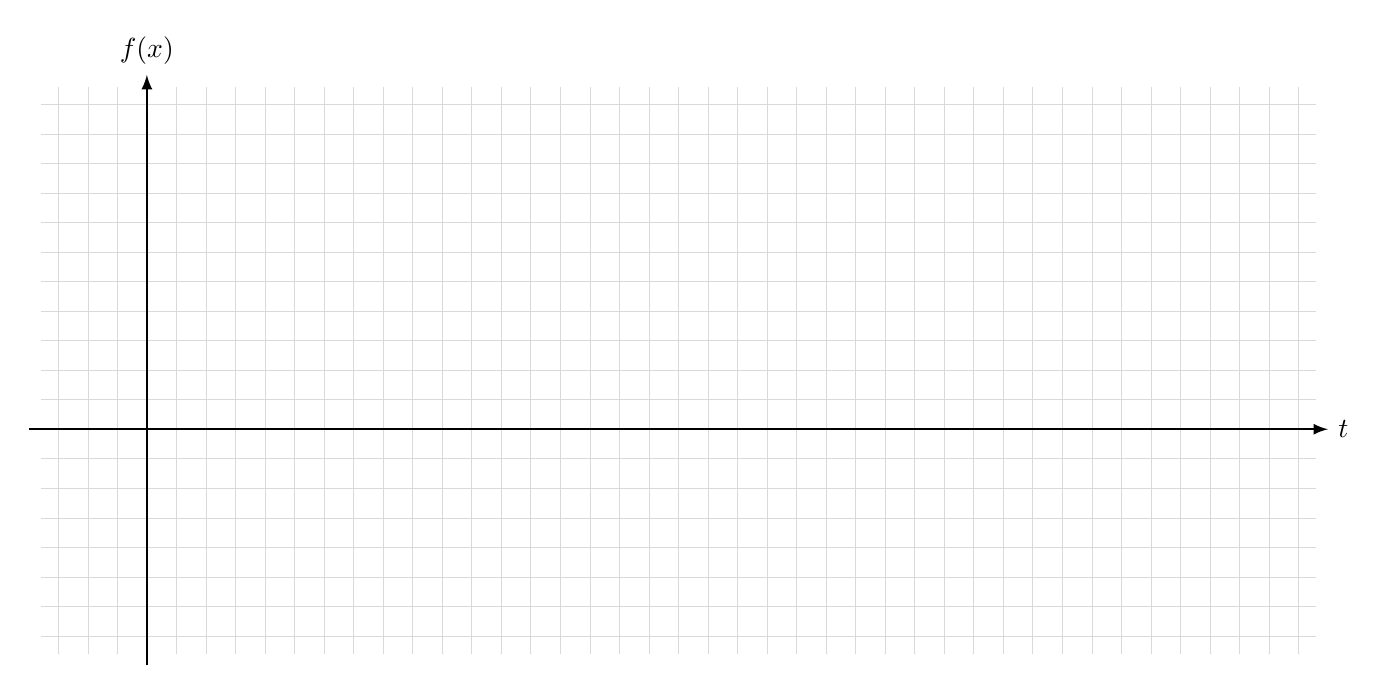
\begin{tikzpicture}[scale = 1.5]
	\draw[step=.25cm,gray!30,very thin] (-3.9,-1.9) grid (6.9,2.9);
	\draw[style = thick,black, -latex] (-4,0) -- (7,0) node[right] {\( t  \)};
	\draw[style = thick,black, -latex](-3,-2) -- (-3,3) node[above]{\( f(x)  \)};
\end{tikzpicture}}
%%

\sisetup{
	locale = DE ,
	per-mode = symbol
}

\pagestyle{headandfoot}

\headrule
\footrule
\firstpageheader{ETIT-1}{\bfseries\Large {Übungsblatt}}{\tdate}
\runningheader{ETIT-1}
{Übungsblatt - }
{\tdate}
\firstpagefooter{ETIT-1}{Seite \thepage\ von \numpages}{\myqr}
\runningfooter{ETIT-1}{Seite \thepage\ von \numpages}{Shah Rrks}

\boxedpoints
%\pointpoints{Punkt}{Punkte}
\pointsinmargin
\marginpointname{\%}

\begin{document}

\section*{Allgemeine Aufgabe}

\begin{questions}
%\question[10] 
Summen ausrechnen

\question[5]
\[\[ \sum_{k=1}^{5} k^2 + 2^{-k} - k\]  \]

\makeemptybox{3in}

\question[5] 
Nullstellen finden 
\begin{parts}
	\part \[ 0,5 x^2 + 20 - 7x = 0  \]
	\makeemptybox{3in}
	%\vspace*{3cm} \newpage
	\part \[ x^3 - 5x^2 + 5x^2 -19x - 30  \]
	\makeemptybox{4in}
\end{parts}
\end{questions}

\section*{Trigonometrie}
\begin{questions}
	

\question[5] 
Wandeln sie folgenden Ausdrücke in eine Kosinus-Funktion 
\[ -7 \cos(t) - 7 \sin(t) \]
\makeemptybox{2in}
\question[5] 
Was versteht man unter Phasor. Erklären sie anhand ein Beispiel.
\makeemptybox{3in}

\drawgraph 

\end{questions}

\section*{Differentialrechnung}
\begin{questions}
	


\question[10]
\begin{figure}[h]
\centering
\includegraphics[width=\textwidth]{images/tunnel_auf.png}
\end{figure}
\end{questions}
\makeemptybox{4in}

\section*{Komplexe Zahlen}
\begin{questions}

\question[10]
\begin{parts}
	\part 
	\begin{align*}
		z_1 &= \frac{2 + 3 i}{ 1 - 2i} \\ 
	\end{align*}
	\makeemptybox{5in}
	\part 
	\begin{align*}
		z_2 &= (1 + i \sqrt (3) )^{12}  \\
	\end{align*}
	\makeemptybox{5in}
\end{parts}
\end{questions}

\end{document}
